\documentclass{article}
\usepackage{graphicx} % Required for inserting images
\usepackage{biblatex}
\usepackage{hyperref}
\addbibresource{references.bib}
\usepackage{amsmath} 
\usepackage{appendix}
\usepackage{subfigure}
\usepackage{graphicx}
\usepackage{float}
\usepackage{algorithmic}
\usepackage{algorithm}
\usepackage{algpseudocode}

\title{AMA546 project}
\author{}
\date{April 2024}

\begin{document}

\maketitle
\section{Introduction}
\subsection{Data Introduction}
Our dataset, titled ``Credit Card Dataset for Clustering'', is sourced from Kaggle. The sample Dataset summarizes the usage behavior of about 9000 active credit card holders during the last 6 months. The file is at a customer level with 18 behavioral variables. These variables cover various aspects such as balance, purchase amounts, frequency of purchases, cash advances, payment details, and credit limits, among others. This dataset is particularly valuable for performing customer segmentation to inform targeted marketing strategies and enhance understanding of consumer spending patterns. The first five samples are shown as follows Fig\ref{fig:dataset}.Here's a brief introduction to some of the key features of the "Credit Card Dataset for Clustering".
\begin{figure}[hbt!]
    \centering
    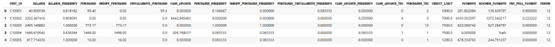
\includegraphics[width=0.8\textwidth]{fig/zya/dataset.png}
    \caption{First five samples from dataset}
    \label{fig:dataset}  % 定义标签
\end{figure}

The feature ``BALANCE'' indicates the amount of money currently available in a customer's credit card account that can be used to make purchases. It reflects the financial flexibility or remaining credit limit of the cardholder. Similarly, ``ONEOFF\_PURCHASES'' is the maximum purchase amount charged to the credit card in a single transaction. It highlights consumer behavior regarding large, one-time expenditures as opposed to smaller or installment-based transactions.
\subsection{Insights from dataset}
We can learn something from these features in Fig\ref{fig:insight}, which is showcasing the financial behaviors and preferences of the credit card holders over the last six months. The ``BALANCE'' indicates that a significant majority (87.76\%) of customers maintain account balances under \$3,750, suggesting a trend towards conservative spending and prudent financial management. And about the ``purchase'' behavior, nearly all customers (99\%) engaged in purchasing activities, with the highest single transaction recorded under \$10,000, illustrating a preference for moderate spending. Additionally, the same percentage prefer installment-based purchases, typically under \$5,000, aligning with a budget-conscious and manageable repayment preference.
\begin{figure}[hbt!]
    \centering
    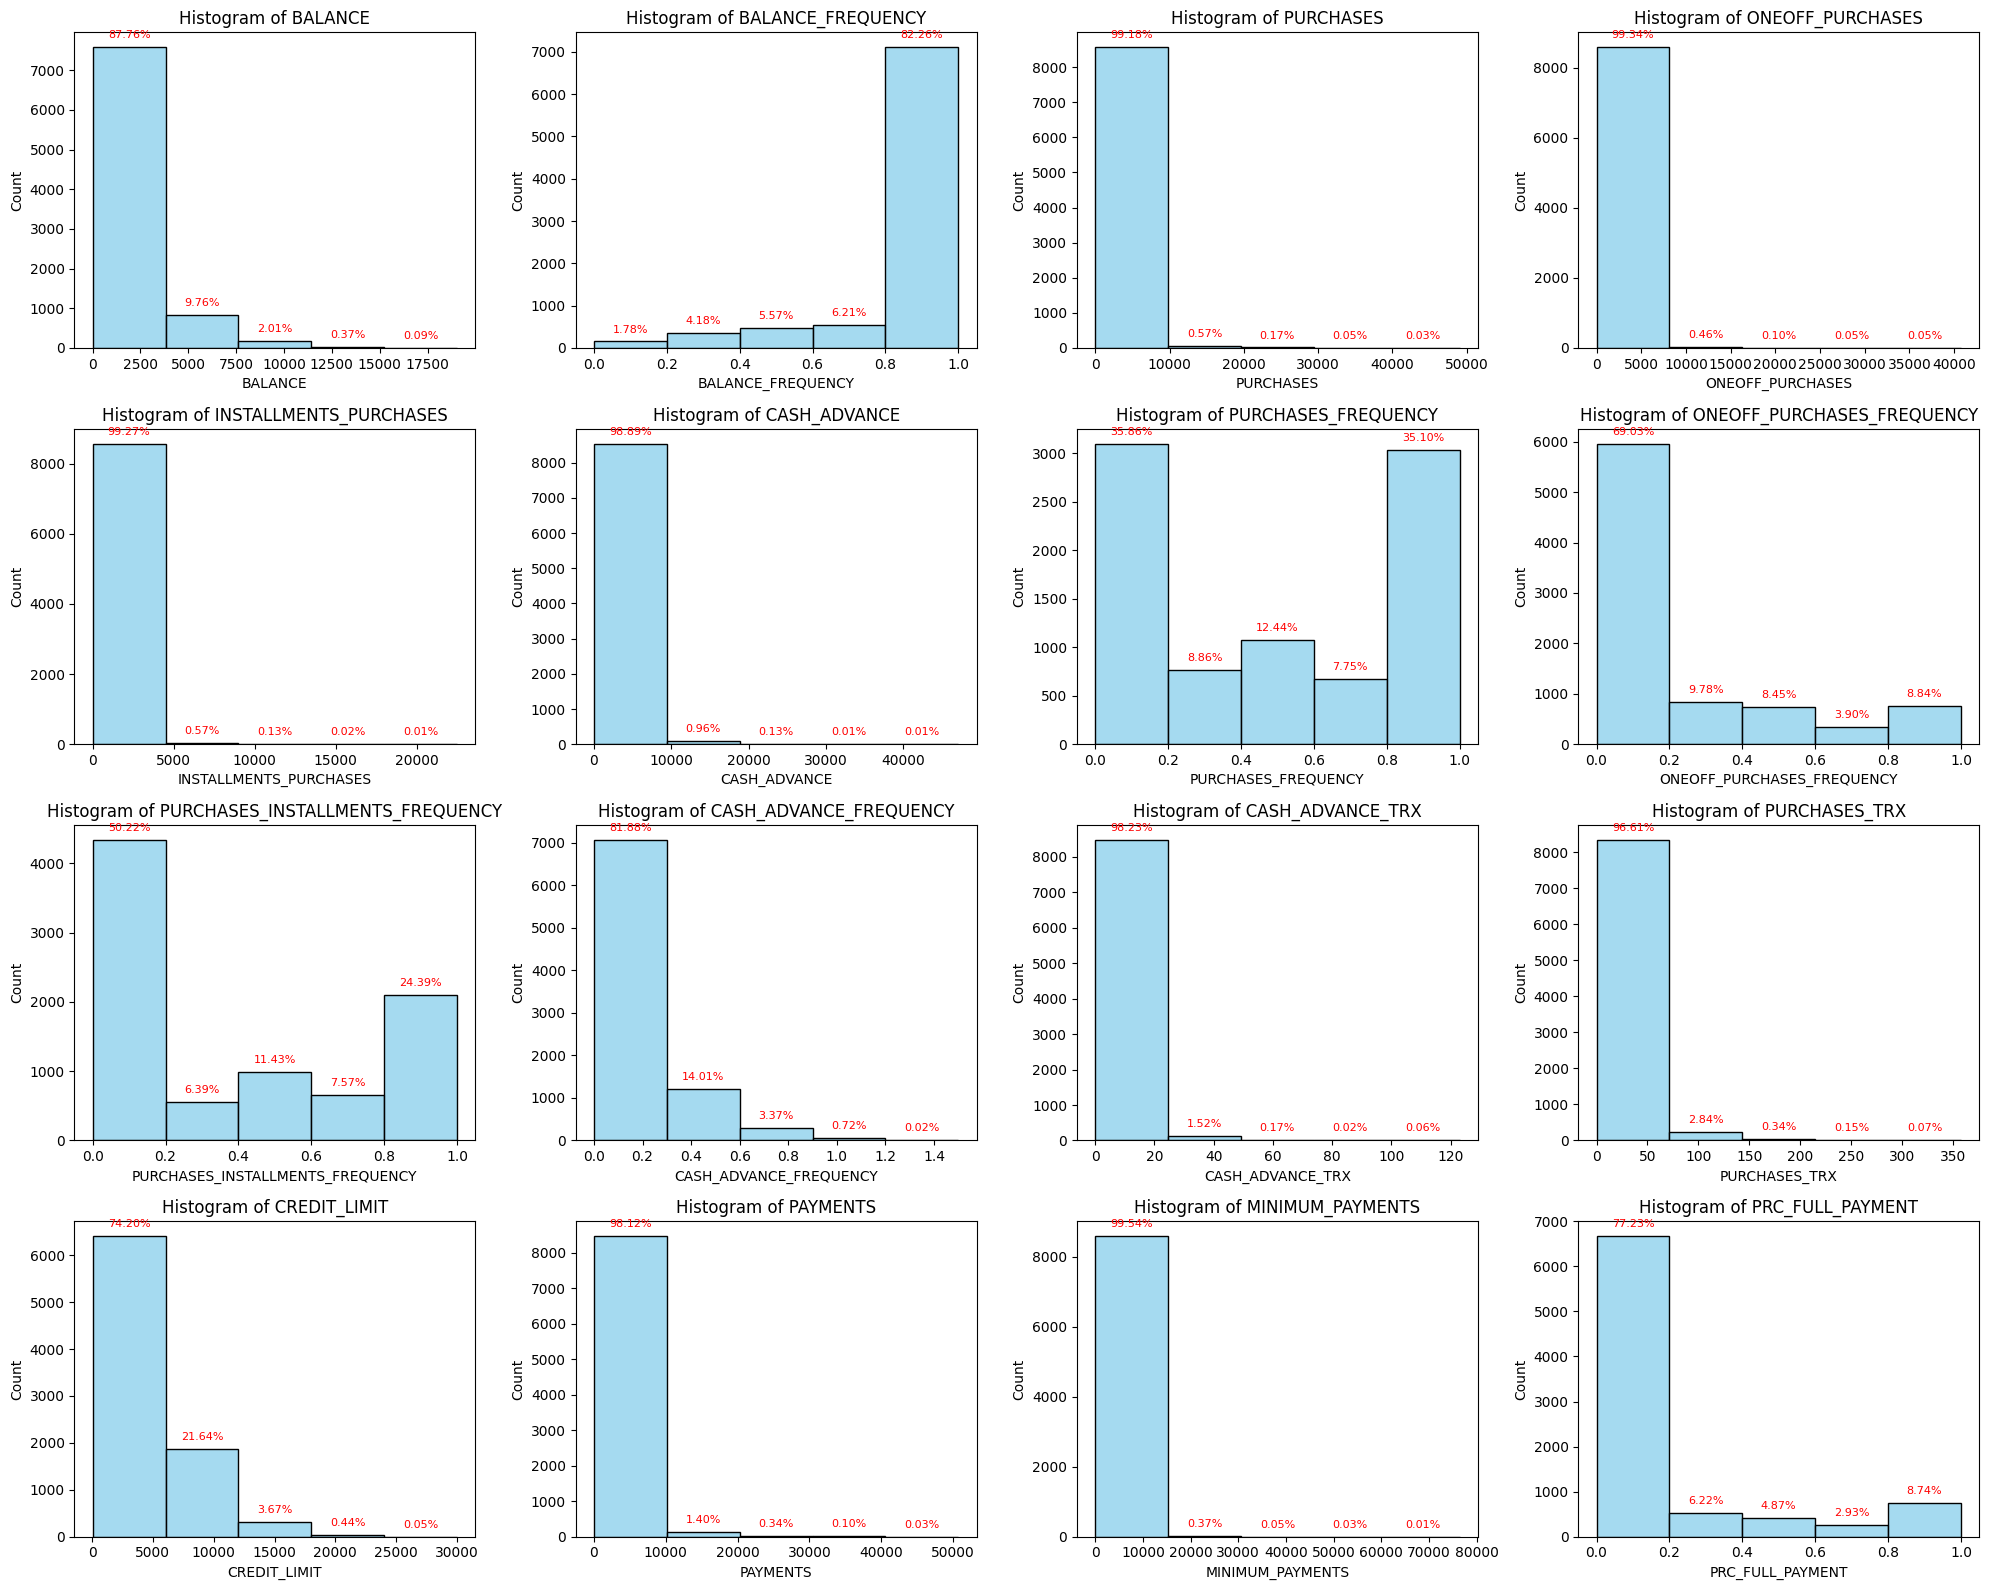
\includegraphics[width=0.8\textwidth]{fig/zya/insight from data.png}
    \caption{Features distribution}
    \label{fig:insight}  % 定义标签
\end{figure}

\section{Data Preprocessing}
\subsection{Data Nomarlization and Missing value}
We have examined the dataset for missing values and found that, as illustrated in the Fig\ref{fig:missing}, the ``MINIMUM\_PAYMENTS'' has 313 missing entries. However, these missing values only account for 3.5\% of the total, which is not significantly impactful. Therefore, we have decided to remove these missing values.
\begin{figure}[hbt!]
    \centering
    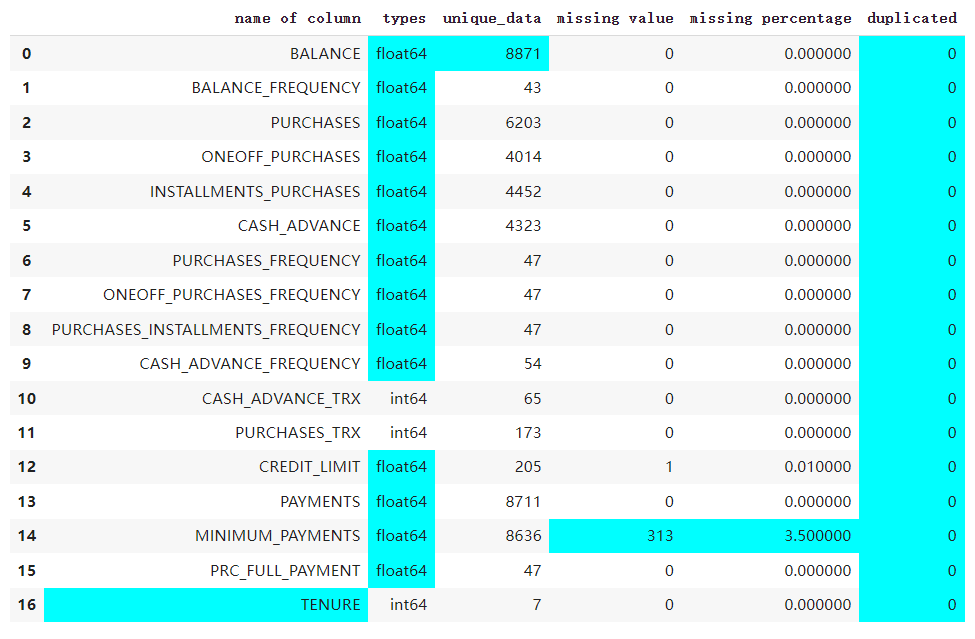
\includegraphics[width=0.8\textwidth]{fig/zya/missing value.png}
    \caption{data describe}
    \label{fig:missing}  % 定义标签
\end{figure}
The we normalize the data, making it satisfy zero mean and unit variance. Data normalization is the process of organizing and standardizing data to improve its consistency and accuracy. This is typically done by scaling the data to a specific range or distribution, making it easier to compare and analyze.
One common method of data normalization is method is z-score normalization, which standardizes the data to have a mean of 0 and a standard deviation of 1. The formula for z-score normalization is:
\begin{equation}
    X_{\text{normalized}} = \frac{X - \mu}{\sigma} 
\end{equation}

where $X$ is the original data, $\mu$ is the mean of the data, $\sigma$ is the standard deviation of the data.

\subsection{Outliers detection}
\label{sec:Outliers detection}
We have conducted outlier processing on the dataset and created Boxplots for all features to display the distribution of the data, marking the outliers. The middle line of each Boxplot represents the median of the feature, while the upper and lower boundaries of the box represent the third and first quartiles (Q3 and Q1, respectively). The length of the box denotes the ``Interquartile Range (IQR),'', which is a measure of data variability. The small dots in Fig\ref{fig:boxplot} depicted in the graph represent outliers, indicating extreme cases in the distribution. Many variables have a substantial number of outliers, for instance, \texttt{BALANCE\_FREQUENCY}, \texttt{ONEOFF\_PURCHASES}, \texttt{PRC\_FULL\_PAYMENT}, and \texttt{TENURE} all have over 1000 outliers. However, removing them is not the best way to solve this problem, so we decided to drop some outliers which are extreme values. 
\begin{figure}[hbt!]
    \centering
    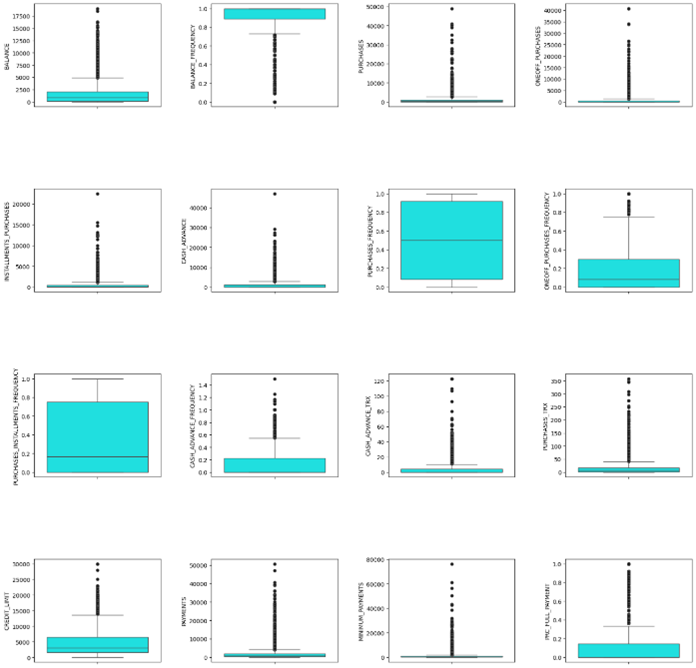
\includegraphics[width=0.8\textwidth]{fig/zya/boxplot.png}
    \caption{Feature boxplot}
    \label{fig:boxplot}  % 定义标签
\end{figure}
For instance, we try to exclude any values in the ``BALANCE'' feature exceeding \$15,000. This decision was made under the presumption that values above this threshold may not accurately represent the typical customer profile and could potentially skew our analysis. Similarly, we removed entries where ``PURCHASES'' exceeded \$40,000, as such high expenditures are atypical and could distort the overall spending patterns we aim to understand. These measures ensure that our dataset more accurately reflects the behavior of an average credit card user.
\subsection{Correcting Skewness in Data}
We can learn from the Fig\ref{fig:skew} that there are many ``right-skewed'' values. The ``MINIMUM\_PAYMENTS'', ``PURCHASES'', ``CASH\_ADVANCE'', and some other features are described as having strong positive skewness. Skewness can introduce several problems when training the dataset. Skewed data can result in clustering algorithms being biased toward the tail, where fewer data points with extreme values exist. The algorithms may incorrectly interpret these extremes as separate clusters or allow these points to unduly influence the shape of the clusters.
\begin{figure}[hbt!]
    \centering
    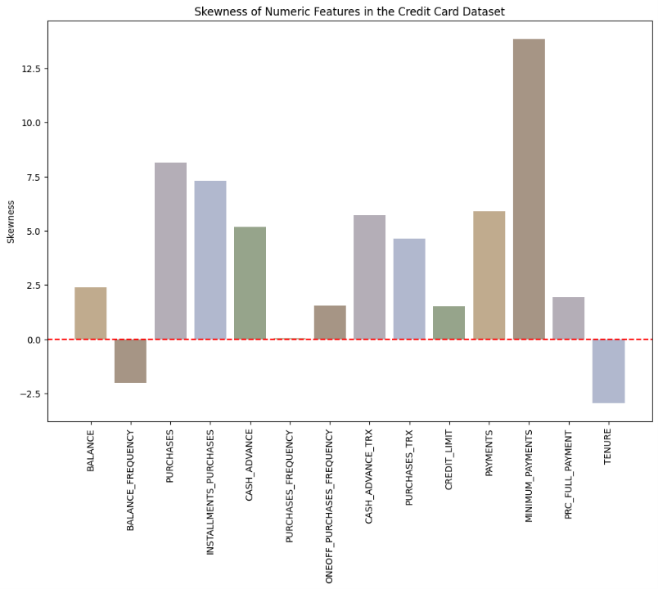
\includegraphics[width=0.6\textwidth]{fig/zya/skewness.png}
    \caption{Feature skewness}
    \label{fig:skew}  % 定义标签
\end{figure}
In our preprocessing efforts to correct for strong positive skewness in our dataset, we have applied a logarithmic transformation to selected features, recognized for their skewness. Before performing the logarithmic transformation, we added a small constant (0.1) to each value within these features. This step ensures that all values are positive and greater than zero, thus making them suitable for the logarithmic function, which is undefined for zero and negative numbers.
\subsection{Correlation analysis}
We have a heatmap to analyze the correlation between the features. A heatmap has been utilized to depict the correlations between different variables within our dataset. This visualization tool is instrumental in identifying and illustrating the degree of linear relationship between pairs of variables. The correlation coefficients range from +1 to -1, where +1 indicates a perfect positive correlation while -1 shows a perfect negative correlation. In our heatmap (Fig\ref{fig:heatmap}), the closer the color is to green, the stronger the positive linear relationship between the variables. Colors approaching brown reflect weaker positive correlations or stronger negative correlations.
\begin{figure}[hbt!]
    \centering
    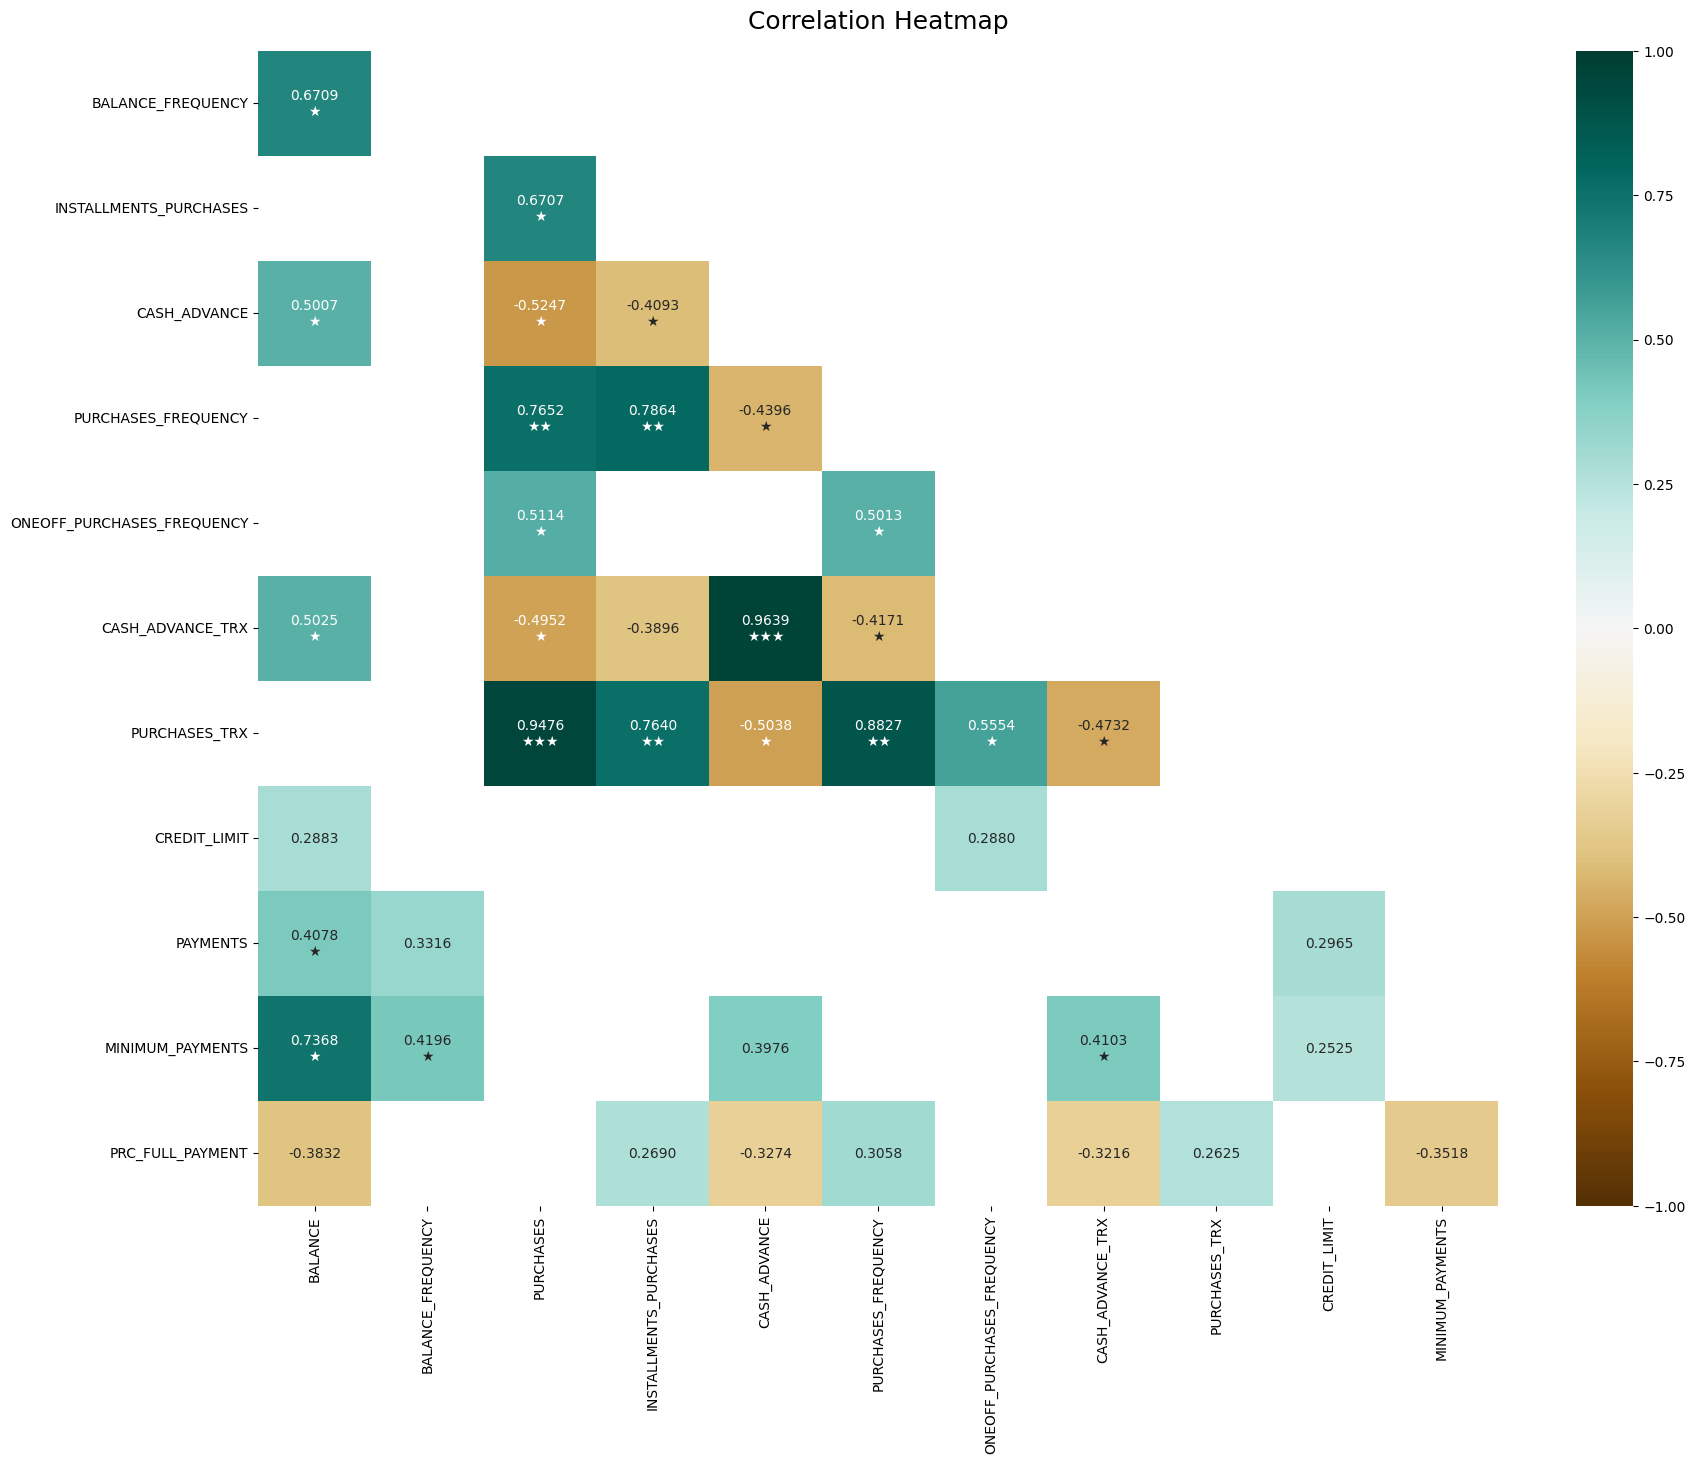
\includegraphics[width=0.8\textwidth]{fig/zya/heatmap.png}
    \caption{Heatmap}
    \label{fig:heatmap}  % 定义标签
\end{figure}

The correlation between ``INSTALLMENTS\_PURCHASES'' and ``PURCHASES\_FREQUENCY'' is 0.7864, indicating a strong positive correlation between these two variables. This suggests that customers who make purchases more frequently tend to prefer using installment payments for these purchases.

\section{Model training and result analysis}
\subsection{K-means}
\subsubsection{The basic of K-means algorithm}
K-means is formally described by algorithm\ref{fig:K-means-al}
\begin{figure}[hbt!]
    \centering
    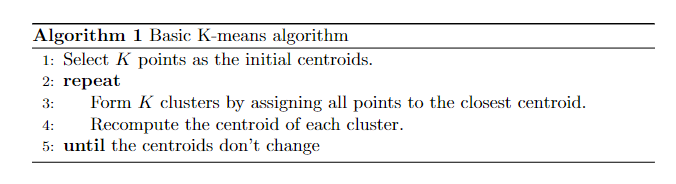
\includegraphics[width=0.8\textwidth]{fig/zya/kal.png}
    \caption{Basic K-means algorithm}
    \label{fig:K-means-al}  % 定义标签
\end{figure}
The steps of the K-means algorithm are as follows. Initially, k random data points are generated as centroids. For each data point, calculate its distance to each centroid and associate the data point with the nearest centroid to form a cluster. Then, recalculate the mean of each cluster to determine new centroids and update them accordingly. Repeat the process by continuing to calculate the distances from each point to the centroids, followed by classification. After classification, compute the means again and update the centroids.This process continues until the centroids no longer change.
The operation of K-means is illustrated in Fig\ref{alg:kmeans}, which shows how,starting from three centroids.
\begin{figure}[hbt!]
    \centering
    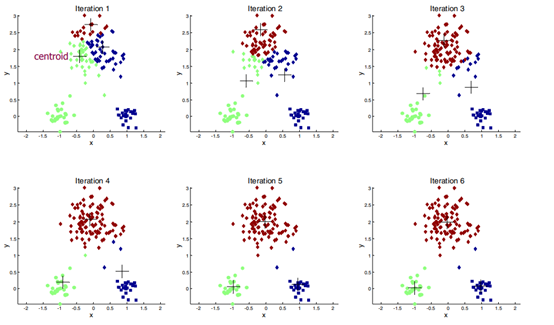
\includegraphics[width=0.5\textwidth]{fig/zya/k-means.png}
    \caption{Using K-means to find three clusters in sample data}
    \label{fig:kmeans}  % 定义标签
\end{figure}


\subsubsection{Clustering}
First, we determine the optimal number of clusters, \( k \), using the elbow method. For each candidate \( k \), we calculate the within-cluster sum of squares (WCSS), which is the sum of squared Euclidean distances of each point from the cluster center.
\begin{equation}
\text{WCSS} = \sum_{i=1}^{k} \sum_{x \in S_i} ||x - \mu_i||^2
\end{equation}
We then plot the relationship between \( k \) and their corresponding WCSS values. Additionally, at \( k = 1 \), the WCSS is at its highest, but as the value of \( k \) increases, the WCSS begins to decrease. The central principle of the elbow method is to choose the last point before the curve levels off as the value of \( k \). On this Fig\ref{fig:Elbow methods to find K}, there is a noticeable “elbow point” at the position of \( k = 3 \) or \( k = 4 \), after which the decline in WCSS slows down. This suggests that adding more clusters does not significantly decrease the WCSS value. Therefore, we choose to set \( k = 4 \).
\begin{figure}[hbt!]
    \centering
    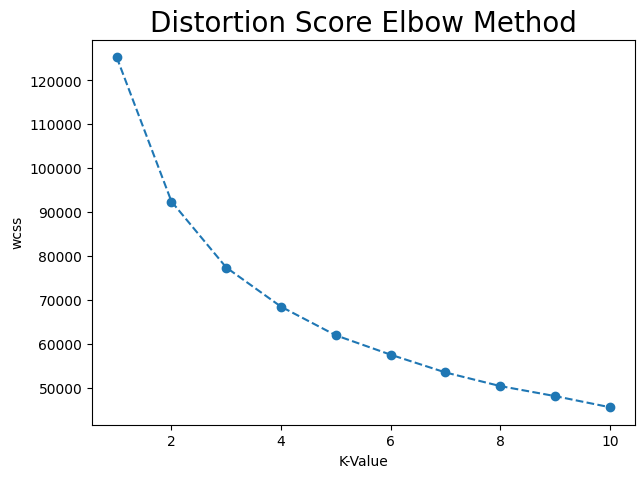
\includegraphics[width=0.6\textwidth]{fig/zya/elbow.png}
    \caption{Using K-means to find three clusters in sample data}
    \label{fig:Elbow methods to find K}  % 定义标签
\end{figure}

We utilized t-SNE to reduce the dimensions to a 2D space for visualization. The Fig\ref{fig:Clusters visualized with t-SNE} below presents a clustering result: there are three distinct clusters in the image, Cluster 0 (blue), Cluster 1 (yellow), and Cluster 2 (purple). Each point represents a data point from the original high-dimensional data, and their positions in the 2D space are intended to preserve the relative distances and structures between the original data points as much as possible.
\begin{figure}[hbt!]
    \centering
    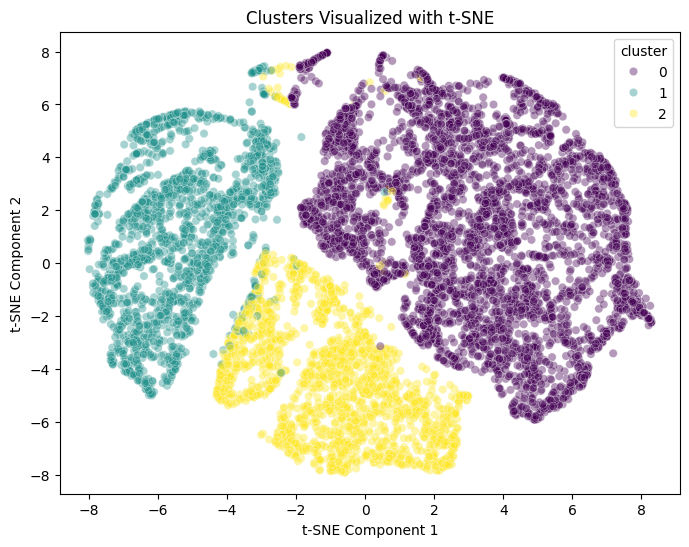
\includegraphics[width=0.8\textwidth]{fig/zya/t-sne-kmeans.png}
    \caption{Clusters visualized with t-SNE}
    \label{fig:Clusters visualized with t-SNE}  % 定义标签
\end{figure}

\subsubsection{Evaluation Metrics}
We used three evaluation metrics: Silhouette Score, Calinski-Harabasz Score, and Davies-Bouldin Score to assess the clustering. The scores are as follows in the table\ref{table:Evaluation Metrics}
\begin{table}[hbt!]
\centering
\caption{Evaluation Metrics}
\begin{tabular}{lcc}
\hline
Evaluation Metrics & \multicolumn{1}{l}{score} \\
\hline
Silhouette Score     & 0.2396 \\
Calinski-Harabasz Score  & 2476.4846 \\
Davies-Bouldin Score          & 1.5397 \\
\hline
\end{tabular}
\label{table:Evaluation Metrics}
\end{table}
.\par

The Silhouette Score of \(0.2396\) is better than \(0\) and is close to \(0.25\), indicating that there is a decent level of cohesion within clusters and separation between clusters, but there is still room for improvement. The Calinski-Harabasz Score of \(2476.4846\) is relatively high, suggesting that there is a high degree of similarity within clusters and a significant difference between clusters, which are signs of good clustering results. The Davies-Bouldin Score of \(1.5397\) is close to \(1.5\); ideally, we want this value to be as low as possible (with the lowest being \(0\)). A score of \(1.5\) means that the points within a cluster are not very compact, or the separation between clusters is not very distinct.
\subsubsection{Result analysis}
First, we transform the cluster centers of the K-means clustering algorithm from the normalized feature space back to the original feature space. The Fig\ref{fig:result1} is shown as follows:
\begin{figure}[hbt!]
    \centering
    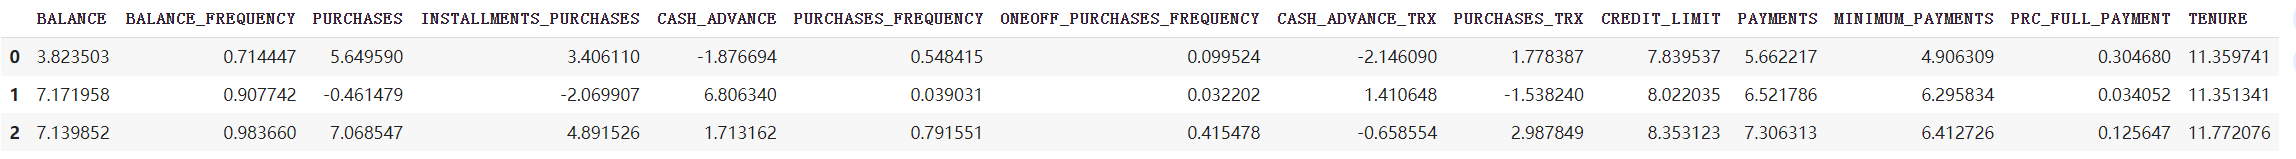
\includegraphics[width=0.8\textwidth]{fig/zya/result1.png}
    \caption{Transform Centroids Back to Original Feature Space}
    \label{fig:result1}  % 定义标签
\end{figure}
.\par
Next, we analyze the characteristic values of each cluster center. In the Fig\ref{fig:result2}, we can see the contribution of characteristic values for each cluster. We can combine this with business analysis to determine the customer characteristics represented by each cluster.
\begin{figure}[hbt!]
    \centering
    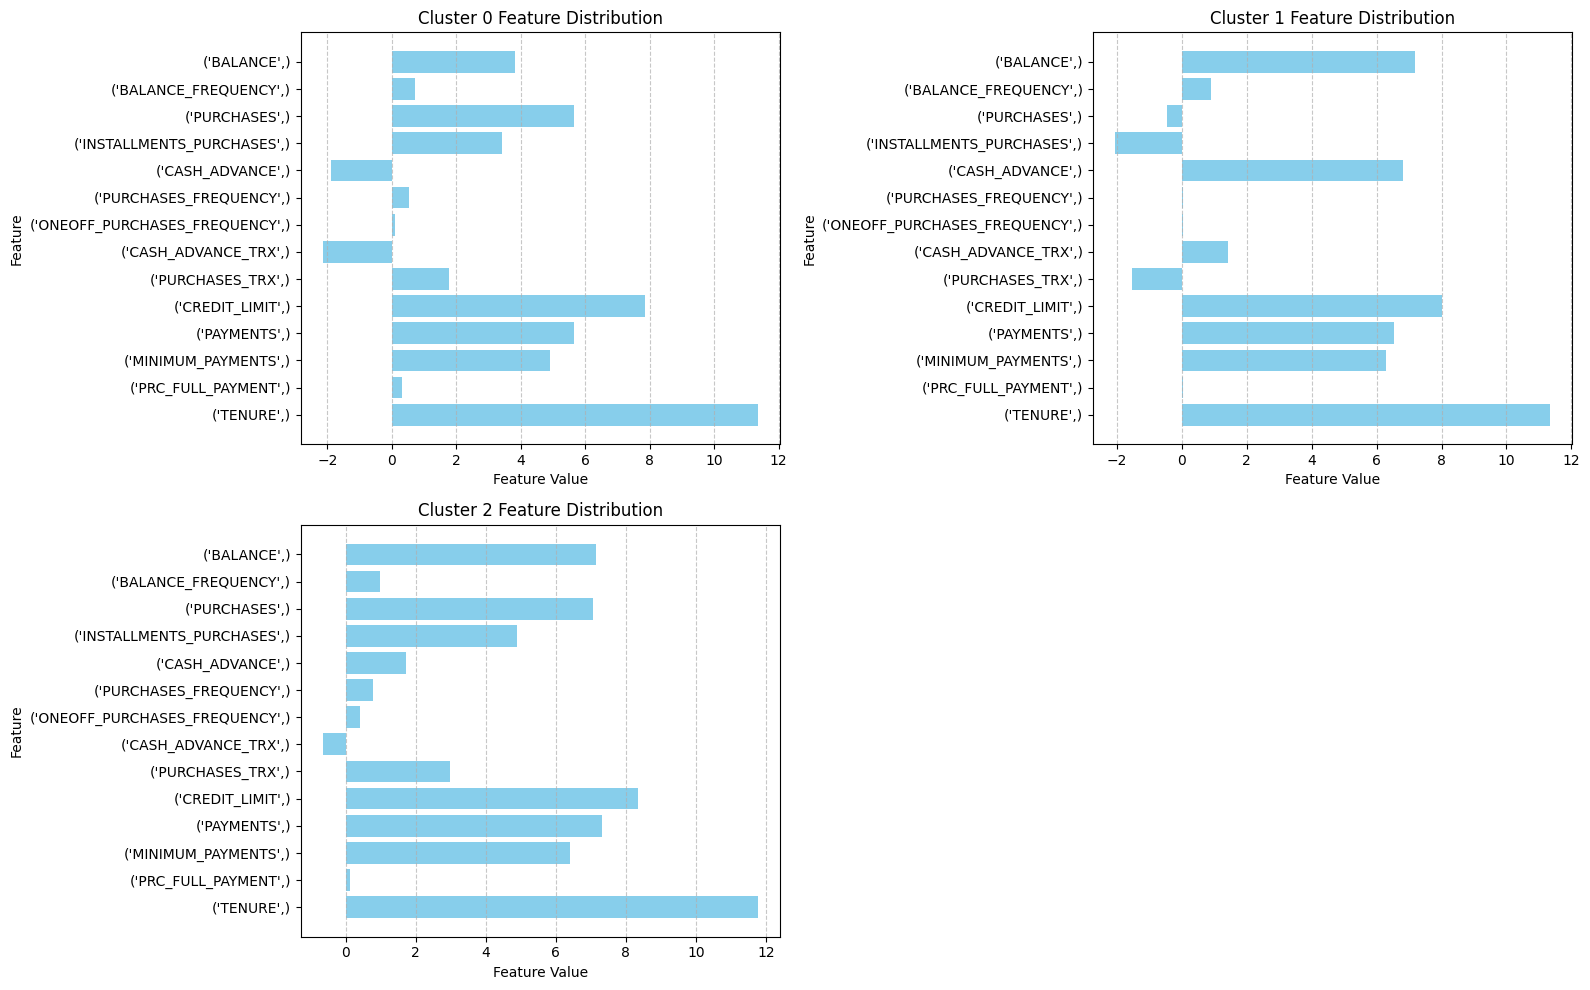
\includegraphics[width=1.2\textwidth]{fig/zya/result2.png}
    \caption{Cluster features}
    \label{fig:result2}  % 定义标签
\end{figure}
.\par
From the Fig\ref{fig:result2}, we can see that the three clusters represent different type of customers.
.\par
\textbf{Cluster 0:} Users with low balances, frequent purchases, and minimal cash advances. These users typically have low credit card balances, indicated by low \texttt{BALANCE}. They exhibit a high frequency of purchases, suggesting regular use of credit cards for transactions, although the amounts may be small. The infrequent use of cash advances might mean that these users prefer paying with their credit cards rather than withdrawing cash. Higher credit limits and payment activity might indicate that these users have good credit and often pay their bills in full. Such users could include young professionals or homemakers who focus more on daily spending and online shopping.

\textbf{Cluster 1:} Users with high balances, low purchase frequency, and high cash advance usage. These individuals hold higher credit card balances, which might indicate a higher financial burden or less frequent debt repayment. Low purchasing activity, especially almost no installment purchases, suggests these users seldom use credit cards for shopping. Frequent use of the cash advance feature indicates that these users might often need cash for daily expenses or emergencies. Such users might be self-employed or small business owners who need to frequently access cash to manage their business or personal finances.

\textbf{Cluster 2:} Users with high balances, active purchasing, and good credit. These users also have high credit card balances but, unlike Cluster 1, they have a high frequency of purchases, particularly installment purchases. This suggests that they may use credit card installment services to buy expensive goods or services. The highest credit limits and payment activities indicate these users likely have high credit ratings and good repayment records. Such users might be high-income professionals accustomed to using credit cards for managing significant expenses while enjoying the benefits and rewards that credit cards offer.

\subsection{new methods}
\subsection{t-sne}
\section{Model training and result analysis}
\subsection{}
\end{document}




    

    